% Modelo de Dissertação do Mestrado em Informática da PUC - Alterado para cumprir a normalização de 2011
%\documentclass[a4paper,brazil,ruledheader,normaltoc,capchap]{abnt}

% Para impressão frente e verso (normalização 2011)
\documentclass[a4paper,brazil,ruledheader,normaltoc,capchap,twoside,openany]{abnt_pucmg_utf8}

% Não esquecer das alterações no arquivo abnt.cls
% Se estiver usando o Kile no Ubuntu o arquivo fica armazenado em /usr/share/texmf/tex/latex/abntex.
% Comentar a linha 967 
% \vspace*{30pt}% - Linha comentada para reduzir o espaçamento entre o topo da página e o título \chapter
% Alterar a linha 1143
% \vspace*{-30pt} % - Parâmetro alterado de 30pt para -30pt para reduzir o espaçamento entre o top da página e o título do apêndice
% Alterar a linha 985
%\vspace*{-30pt}\par % - Parâmetro alterado de 0pt para -30pt para reduzir o espaçamento entre o top da página e o título \chapter*
% Alterar a linha 991
% Parâmetro alterado de 45pt para 30pt para reduzir o espaçamento entre o texto e o título \chapter*

% Não esquecer das alterações no arquivo acronym.sty
% Se estiver usando o Kile no Ubuntu o arquivo fica armazenado em /usr/share/texmf-texlive/tex/latex/acronym
% Alterar a linha 225
%\item[\protect\AC@hypertarget{#1}{\acsfont{\normalfont{#2}}} --] #3% - Inserir separador entre acrônimo/descrição e remover o negrito com o normalfont

% Pacote para definir explicitamente as margens das páginas
\usepackage[a4paper,left=3cm,right=2cm,top=3cm,bottom=2cm]{geometry}

%\usepackage{units}
% Utilize da seguinte forma \unit[78,6]{mA}

% Pacote para gerenciar siglas
\usepackage[printonlyused]{acronym}

% Merge em duas células (linhas diferentes)
\usepackage{multirow}

% Pacote para citação e referências seguindo ABNT no sistema (AUTOR, Data)
%\usepackage[alf, bibjustif,abnt-emphasize=bf]{abntcite}
%\usepackage[alf, abnt-emphasize=em, abnt-thesis-year=title]{abntcite}
\usepackage[alf]{abntex2cite}
% @article An article from a journal or magazine 
% @inproceedings An article in a conference proceedings
% Força que o tipo de ênfase no nome do simpósio seja em caixa alta
\renewcommand{\emph}{\textsc}

% Pacote para múltiplos arquivos .bib
\usepackage{multibib}
%\newcites{pub}{Refer\^encias das publica\c{c}\~oes}

% Pacote de adequação do formato ABNT para normas da PUCMinas
\usepackage{abnt-PPGInf-PUCMG}

% Pacotes utilitários
\usepackage{graphicx}

% Pacote para fixar a figura no local desejado
\usepackage{float}

% Pacote para adicionar simbolos as informações de rodapé
\usepackage[symbol]{footmisc}

\usepackage[all]{xy}
%\usepackage[tight]{subfigure}	% Permite a criação de subfiguras
\usepackage{url,amsmath}	% Permite melhorias na codificação de fórmulas
%\usepackage{amsthm}		% Permite melhorias na escrita de teoremas
\usepackage{amssymb}		% Permite utlização de simbolos matemáticos avançados

\usepackage[portuguese, linesnumbered, ruled, vlined]{algorithm2e}
\usepackage{algorithmic} 	% para algoritmos
\usepackage{listings} 		% para importação de código-fonte

% Alterar o espaçamento da margem no algoritmo
\setlength{\algomargin}{1em}

\usepackage{setspace}

% Pacote para rotação de tabelas/figuras
\usepackage{rotating}

% Pacotes para criação de cronograma/tabela colorida
\usepackage{color}
\usepackage{array}
\usepackage{longtable}
\usepackage{colortbl}
%\definecolor{lightgray}{gray}{0.9}

% Pacote para possibilitar o uso do setboolean para forçar formatos de página diferentes do padrão do documento
\usepackage{ifthen}

% Para inserir captions (nova normalização 2011)
\usepackage[size=normalsize,labelfont=bf,textfont={bf},labelsep=endash]{caption}
\captionsetup[subfloat]{labelfont=bf,textfont={bf}}

% Usado para reduzir espaçamentos entre itens (alíneas, enumerações) com o compactitem
\usepackage{paralist}

% Alterar para sequencial a numeração de figuras e tabelas
\captionsetup{figurewithin=none}
\captionsetup{tablewithin=none}

\setlength{\LTcapwidth}{\textwidth}

% Para o subsubsection aparecer no sumário 
\setcounter{tocdepth}{3}
\setcounter{secnumdepth}{3}

% Para inserir referências via links - não funciona para abntex
%\usepackage[colorlinks=true,pdfstartview=FitV,linkcolor=blue,citecolor=blue,urlcolor=blue,hyperindex,pagebackref=true,pdftex,breaklinks]{hyperref}
%\usepackage[pdftex]{hyperref}

% Para criar lista de gráficos
\floatstyle{plaintop}
\newfloat{grafico}{H}{loq}
\restylefloat*{grafico}
\floatname{grafico}{Gráfico} 

% Para gerar subfiguras usando o subfloat
\usepackage{subfig}
\newsubfloat[position=bottom,listofformat=subsimple]{grafico}

% define estilo de posicionamento na caixa
\newsavebox{\leftfig}
\newsavebox{\rightfig}

%\renewcommand{\ALG@name}{Algoritmo}
%\renewcommand{\listalgorithmname}{Lista de Algoritmos}

% Configuração de código-fonte
\lstset{extendedchars=\true, % permite acentos
 inputencoding=utf8,
 literate={\$}{{\$}}1,
 commentstyle=\it, % deixa os comentários em itálico
 stringstyle=\bf, % não lembro o que faz, mas está funcionando
 belowcaptionskip=5pt, % não lembro o que faz, mas está funcionando
 numbers=left, % coloca a numeração na esquerda
 stepnumber=1, % passos da numeração
 firstnumber=1, % primeira linha
 numberstyle=\tiny, % tamanho da fonte da numeração
 breaklines=true, % permitir quebra de linha
 frame=tb, % borda em cima e em baixo
 basicstyle=\footnotesize, % estilo básico
 stringstyle=\ttfamily, % não lembro o que faz, mas está funcionando
 showstringspaces=false, % não mostrar os espaços
 mathescape, % não lembro o que faz, mas está funcionando
 tabsize=3 % tamanho da tabulação
}
\renewcommand{\lstlistingname}{Código}
\renewcommand{\lstlistlistingname}{Lista de Códigos}
%\citeoption{abnt-etal-cite=1, abnt-and-type=e}

% the bibtex style generates this command, but it's not defined
%\newcommand{\optionaltextstyle}{}

%%\pdfinfo{%
%%  /Title    (TITULO DA DISSERTACAO)
%%  /Author   (Nome do aluno)
%%  /Creator  (Nome do aluno)
%%  /Producer (Kile - an Integrated LaTeX Environment - %%Version 2.0.85)
%%  /Subject  (Dissertação de Mestrado)
%% /Keywords (Palavras chave)
%%}

% PRÉ-TEXTUAIS %%
\begin{document}

% Para forçar que elementos pré-textuais (da capa até o sumário) sejam impressos no anverso da folha
\setboolean{@twoside}{false}

\autor{André Dias dos Santos Júnior}

% Coloque o título em caixa alta. É o padrão da PUC.
% Vá no arquivo abnt-PPGInf-PUCMG.sty e procure por esse título (linha 575). Altere para o seu título em caixa alta. Isso será utilizado na folha de aprovação.
\titulo{LOCALIZAÇÃO E CLASSIFICAÇÃO DE OBJETOS USANDO REDES NEURAIS CONVOLUTIVAS}

\orientador[Orientador:]{Dr. Zenilton Kléber Gonçalves do Patrocínio Júnior}

% Se não tiver, co-orientador, comente a próxima linha.
%\coorientador[Co-orientador:]{Professor}

% Texto
\comentario{Monografia apresentado ao Curso de Bacharelado em Engenharia de Computação da Pontifícia Universidade Católica de Minas Gerais,
como requisito parcial para obtenção do título de Bacharel em Engenharia de Computação.}


% Instituição
\instituicao{Bacharelado em Engenharia de Computação \par Instituto de Ciências Exatas e Informática \par Pontifícia Universidade Católica de Minas Gerais}

% Local
\local{Belo Horizonte}

% Data
\data{31 de Maio de 2019}
\capa
%Para forçar que a ficha catalográfica seja impressa no verso da folha de aprovação
%\setboolean{@twoside}{true}
\setboolean{@openright}{true}
\setboolean{@twoside}{false}
% Gera a folha de rosto
\folhaderosto

% Ficha catalográfica
% Ficha catalográfica
% INCLUIR O ARQUIVO PDF GERADO PELA BIBLIOTECA COMO FIGURA.
\begin{figure}[h!]
	\vspace*{-3.3cm}
	\hspace*{-3cm}
%	% Suponha o nome do arquivo em pre-texto/ficha-catalografica/fichacatalografica.pdf
	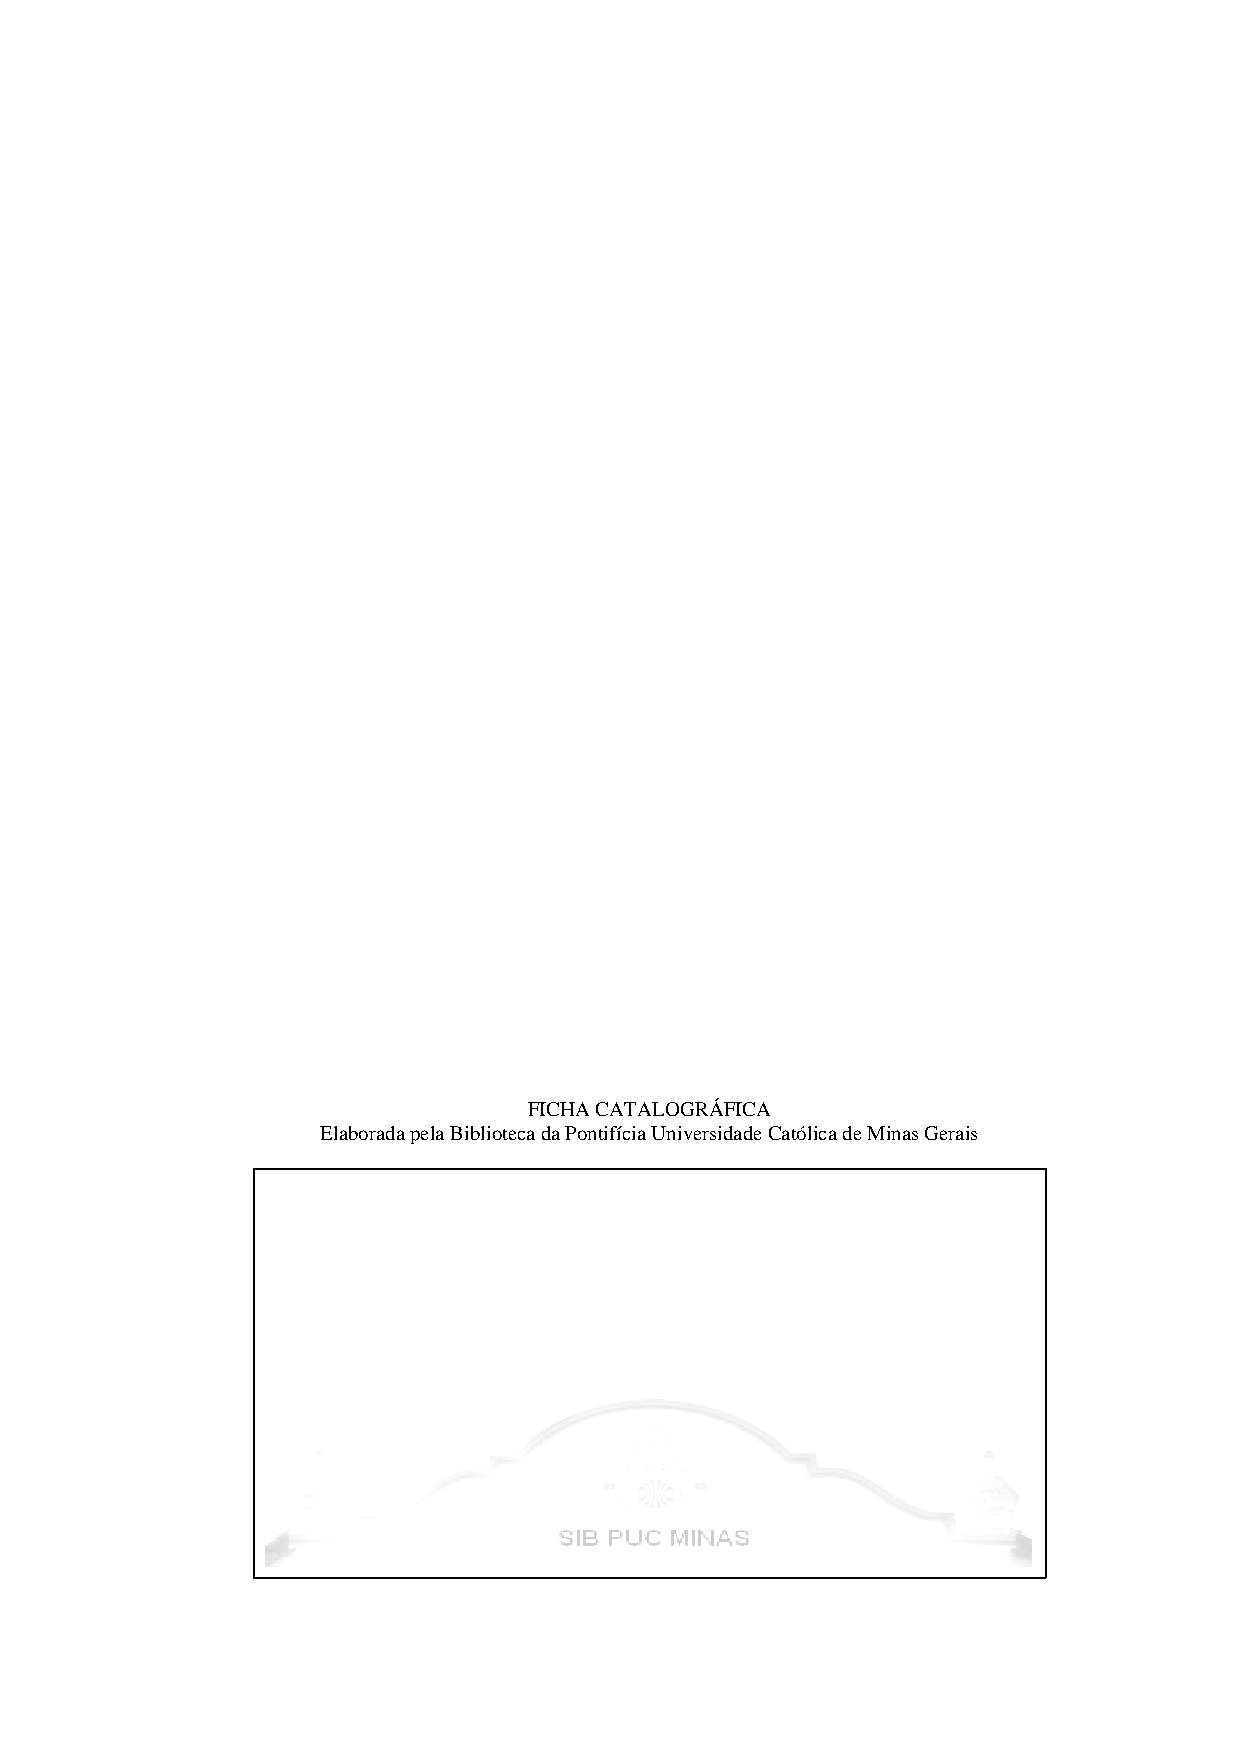
\includegraphics{pre-texto/ficha-catalografica} 
	\newpage
\end{figure}

% Para forçar que elementos pré-textuais (da capa até o sumário) sejam impressos no anverso da folha
\setboolean{@twoside}{false}
% Folha de aprovação
% Termo de Aprovação

% Texto da aprovação
\textoaprovacao{Monografia apresentado ao Curso de Bacharelado em Engenharia de Computação da Pontifícia Universidade Católica de Minas Gerais,
	como requisito parcial para obtenção do título de Bacharel em Engenharia de Computação.}

% Primeira assinatura
\primeiroassina{Prof. Dr. Zenilton Kléber Gonçalves do Patrocínio Júnior -- PUC Minas}

% Segunda assinatura
\segundoassina{Prof. Dr. Membro interno -- PUC Minas}

% Terceira assinatura
\terceiroassina{Prof. Dr. Membro externo -- Instituicao}

% Quarta assinatura
%\quartoassina{}

% Data da defesa
\localdia{Belo Horizonte, 4 de Dezembro de 2020.}

% Gera o termo de aprovação
\termodeaprovacao	

% Dedicatória
% Dedicatória
\newpage

% Espaçamento do topo da página até o texto da dedicatória
\vspace*{22cm}

% Espaçamento na esqueda
\hspace{8cm}\begin{minipage}{.60\textwidth}
            \textit{À minha amada avó, que sempre me apoiou.}
            \end{minipage}

% Agradecimentos
% Agradecimentos
%\chapter*{Agradecimentos}
\begin{center}
	\normalsize
	\textbf{AGRADECIMENTOS}
	
	Em primeiro lugar, agradeço a Deus, que me deu forças para prosseguir, mediante aos obstáculos.
	
	Agradeço também à minha avó por ter me apoiado incondicionalmente e por ter sempre acreditado em mim.
	
	Agradeço também à minha mãe por ser um suporte sólido e por sempre me apoiar quando precisei.
	
	Agradeço também ao meu orientador, o professor Zenílton pelo apoio, a presença, o auxílio prestado e pelo aprendizado ao longo da minha jornada.
	
	Agradeço ao meu pai por torcer por mim e pelas orações.
	
	E agradeço à todos os familiares e amigos que, de alguma forma me auxiliaram ao longo deste caminho
\end{center}

 

% Epígrafe
% Epígrafe
\newpage

% Espaçamento entre topo da página e texto da epígrafe
\vspace*{10cm}
% Espaçamento na esqueda
\hspace{4cm}\begin{minipage}{.51\textwidth}

% Texto da epígrafe
\textit{``E fazendo que se aprende a fazer aquilo que se deve aprender a fazer.'' }

%Nome do autor
\begin{flushright}\itshape Aristoteles \upshape\end{flushright}

\end{minipage}

% Resumo
% Resumo
\begin{resumo}
% Diminuir espaçamento entre título e texto
\vspace{-1cm}

% Texto do resumo: sem paragrafo, justificado, com espaçamento 1,5 cm
\onehalfspacing

\noindent 
   Atualmente há um expressivo crescimento no volume de conteúdo visual, como imagens e vídeos, disponíveis para utilização. As informações contidas em imagens e vídeos são utilizadas pelas mais variadas áreas da sociedade, como médica, industrial e, até mesmo, para fins pessoais. Todos os dias são estudados novos métodos computacionais para fazer recuperação e análise de imagens. Dois métodos que tem sido frequentemente estudados em conjunto são a localização e classificação de objetos. Arquiteturas de \textit{Deep Learning} podem ser implementadas para fazer localização e classificação de objetos, obtendo bons resultados, porém possuem certas limitações como o tamanho dos objetos ou a resolução da imagem. Para contornar essa limitação, pretende-se acrescentar camadas de convolução ao final de uma rede convolutiva densa para fazer a localização dos objetos de diversos tamanhos de forma mais apurada. %Após as camadas finais de Convolução, serão acrescentadas camadas de Deconvolução, para aumentar a escala dos mapas, e decodificar os resultados das convoluções de forma a aumentar  precisão do resultado.

% Espaçamento para as palavras-chave
\vspace*{.75cm}

% Palavras-chave: sem parágrafo, alinhado à esquerda
\noindent Palavras-chave: \textit{Deep Learning}, Localização, Classificação, Convolução.\\ %, Deconvolução.\\
% Segunda linha de palavras-chave, com espaçamento.
%\indent\hspace{2cm}Palavra.

\end{resumo}

% Abstract
% Abstract
\begin{abstract}
% Diminuir espaçamento entre título e texto
\vspace{-1cm}
% Texto do resumo, em inglês: sem paragrafo, justificado, com espaçamento 1,5 cm
\onehalfspacing
\noindent
  Texto do resumo, em ingles.

% Espaçamento para as palavras-chave
\vspace*{.75cm}

% Palavras-chave: sem parágrafo, alinhado à esquerda
\noindent Keywords: . \\
% Segunda linha de palavras-chave, com espaçamento.
%\indent\hspace{1.4cm} Keyword.

\end{abstract}

\makeatletter
\renewcommand\numberline[1]{
	\leftskip 0em
	\rightskip 1.6em
	\parfillskip -\rightskip
	\parindent 0em
	\@tempdima 2.0em
	\vspace{0em} \advance\leftskip \@tempdima \null\nobreak\hskip -\leftskip
	FIGURA \normalfont #1 -- }
\makeatother

% Lista de figuras
\listoffigures

\makeatletter
\renewcommand\numberline[1]{
	\leftskip 0em
	\rightskip 1.6em
	\parfillskip -\rightskip
	\parindent 0em
	\@tempdima 2.0em
	\vspace{0em} \advance\leftskip \@tempdima \null\nobreak\hskip -\leftskip
	TABELA \normalfont #1 -- }
\makeatother

% Lista de tabelas
\listoftables

\makeatletter
\renewcommand\numberline[1]{
	\leftskip 0em
	\rightskip 1.6em
	\parfillskip -\rightskip
	\parindent 0em
	\@tempdima 2.0em
	\vspace{0.5em} \advance\leftskip \@tempdima \null\nobreak\hskip -\leftskip
	GRÁFICO \normalfont #1 -- }
\makeatother

% Lista de graficos
%\listof{grafico}{Lista de Graficos}

% Lista de siglas
% Lista de Abreviaturas e Siglas
%\chapter*{Lista de Abreviaturas e Siglas}
\chapter*{Lista de Abreviaturas e Siglas}

% Mantenha sempre em ordem alfabética.

\begin{acronym}
\acro{CNN} {\textit{Convolutional Neural Networks} - Redes Neurais Convolucionais}
\acro{COCO} {\textit{Common Objects in Context}}
\acro{CVPR} {\textit{Conference on Computer Vision and Pattern Recognition} - Conferência de Visão Computacional e Reconhecimento de Padrões}
\acro{DBN}{\textit{Deep Belief Networks}}
\acro{DeconvNet} {\textit{Deconvolutional Network}}
\acro{DenseNet}{\textit{Densely Connected Convolutional Networks} - Redes Convolutivas Densamente conectadas}
\acro{DSSD}{\textit{Deconvolutional Single-Shot Detector}}
\acro{FCN}{\textit{Fully Convolutional Network} - Rede Completamente Convolucional}
\acro{FPS} {\textit{Frames Per Second} - Quadros Por Segundo}
\acro{IA} {Inteligência Artificial}
\acro{ILSVRC} {\textit{ImageNet Large Scale Visual Recognition Challenge}}
\acro{mAP}{\textit{Mean Average Precision} - Média da precisão Média}
\acro{MLP} {\textit{Multi-Layer Perceptron}}
\acro{MSE} {\textit{Mean Squared Error} - erro quadrático médio}
\acro{PASCAL VOC} {\textit{PASCAL Visual Object Classes}}
\acro{Pixels} {Pontos em uma imagem rasterizada ou menor elemento mostrado no dispositivo de saída de vídeo}
\acro{RBM}{\textit{Restricted Boltzmann Machines}}
\acro{R-CNN}{\textit{Regions with CNN features}}
\acro{ReLU}{\textit{Rectified Linear Unit} - Ativação Linear Retificada}
\acro{ResNet}{\textit{Residual Network} - Rede Neural Residual}
\acro{RNA} {Rede Neural Artificial}
\acro{RPN}{\textit{Region Proposal Network}}
\acro{SSD} {\textit{Single-Shot multi-box Detector}}
\acro{YOLO} {\textit{You Only Look Once} - você só olha uma vez}
\end{acronym}

\makeatletter
\renewcommand\numberline[1]{#1\hspace{0.8em}}
\makeatother

% Altera para espaçamento simples a partir daqui
\singlespacing

% Sumário
\tableofcontents

% Altera para espaçamento 1,5 a partir daqui
\onehalfspacing

%% TEXTUAIS 
% Para forçar que elementos textuais e pós-textuais sejam impressos no anverso e verso das folhas
\setboolean{@twoside}{true}
% Altere o número da página para o correto. Conte todas as páginas frente e verso, menos a capa, nclusive a ficha catalográfica até a página do primeiro capítulo.
\setcounter{page}{8}

% Capítulos
% Para forçar que o capítulo de introdução comece no anverso
% Nome do capítulo
\chapter{Introdução}
% Label para referenciar
\label{cap:1}

% Diminuir espaçamento entre título e texto
\vspace{-1.9cm}

Atualmente há um expressivo crescimento no volume de conteúdo visual, como imagens e vídeos, disponíveis para utilização. Podemos vincular este fato à popularização das tecnologias produtoras destes tipos de conteúdo, como celulares com câmeras, bem como a expansão da Internet e seus canais de comunicação, que utilizam de imagens e vídeos para divulgação de informações. As informações contidas em imagens e vídeos são utilizadas pelas mais variadas áreas da sociedade, como médica, industrial e, até mesmo, para fins pessoais e de entretenimento.

O processamento digital de imagens contribui para a descoberta de informação visual contida em imagens e vídeos. Um dos problemas de processamento digital de imagens amplamente explorados na literatura é o problema de classificação e localização de objetos em imagens. \citeonline{everingham-2015} definem que o problema de classificação consiste em responder para cada classe de objeto se existe ou não uma ou mais instâncias daquele objeto na imagem e, o problema de localização consiste em dizer onde na imagem estão as instâncias dos objetos reconhecidos pelo classificador.

  \begin{figure}[H]
% Alterar espaçamentos antes e depois do caption
  \setlength{\abovecaptionskip}{0pt}
  \setlength{\belowcaptionskip}{0pt}
% Caption
  \caption[Exemplo de Classificação e Localização]{Exemplo de Classificação e Localização de Objetos}
  \centering
  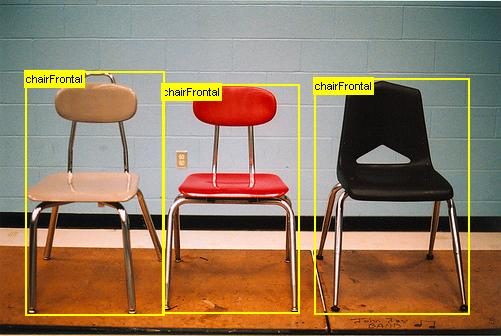
\includegraphics[width=.9\textwidth]{imagem/0x_classdetec.jpg}
% Caption centralizada
  \captionsetup{justification=centering}
  \captionfont{\small{\textbf{\\Fonte: \citeonline{everingham-2015}.}}}	
  \label{fig:exemploclassdet}
  \end{figure}

A Figura \ref{fig:exemploclassdet} mostra exemplos de como devem ser as saídas de um algoritmo de classificação e localização de objetos. Os retângulos destacados em torno dos objetos são resultados do algoritmo de localização que determina que dentro daquela região existe um objeto de interesse e os rótulos destacados em cima dos retângulos são os resultados do algoritmo de classificação, que determina que o objeto contido dentro da região pertence àquela classe.

O uso das \ac{CNN} tem se tornado cada vez mais populares, principalmente em alguns dos problemas clássicos de processamento de imagens. A primeira abordagem desse tipo foi proposta por \citeonline{fukushima-1980} para fazer reconhecimento de caracteres escritos a mão. Mais tarde, \citeonline{lecun-1998} desenvolveram uma arquitetura de \ac{CNN} para a mesma tarefa e obtiveram uma acurácia de $70\%$, sendo essa muito superior aos resultados obtidos por qualquer outro classificador utilizado até então.

%%% p1 Escrever sobre os resultados obtidos pelas CNNs em classificação de imagens
Contudo, as \ac{CNN} só passaram a ser utilizadas com mais frequência algum tempo depois. \citeonline{deng-2009} lançaram o ImageNet, uma base de dados de larga escala com mais de 14 milhões de imagens anotadas manualmente divididas em mais de 22 mil classes diferentes. Essa base de imagens pode ser usada para as tarefas de classificação, detecção e localização de objetos. Além disso, \citeonline{deng-2009} também lançaram o \ac{ILSVRC}, uma competição global anual, aonde os competidores são avaliados nas tarefas de classificação de imagens, detecção de objetos e localização de objetos. \citeonline{krizhevsky-2012} alcançaram o melhor resultado no \ac{ILSVRC} de 2012 usando a AlexNet - uma \ac{CNN} - e desde então, as \ac{CNN}s obtém sempre os melhores resultados nos desafios.

Em \citeyear{he-2016}, \citeauthor{he-2016} propuseram a \ac{ResNet} que introduziam o conceito de \textit{skip connection}. Uma \textit{skip connection} é quando a camada $C_n$ além de se conectar com a camada $C_{n+1}$ ela se conecta com outra mais a frente - no caso da \textit{\ac{ResNet}}, a camada $C_{n+3}$. Sendo assim, a camada $C_{n+3}$ recebe em suas entradas uma junção das saídas de $C_{n}$ e $C_{n+2}$. Essa combinação de entradas na \ac{ResNet} foi feita como uma soma de matrizes. A Figura \ref{fig:blocoresidual} mostra um exemplo de \textit{skip connection} na \textit{\ac{ResNet}}.

\begin{figure}[H]
	% Alterar espaçamentos antes e depois do caption
	\setlength{\abovecaptionskip}{0pt}
	\setlength{\belowcaptionskip}{0pt}
	% Caption
	\caption[Exemplo de bloco residual]{Exemplo de bloco residual}
	\centering
	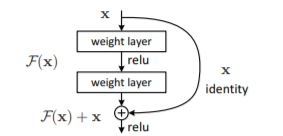
\includegraphics[width=.5\textwidth]{imagem/0x_resnet_arch.jpg}
	% Caption centralizada
	\captionsetup{justification=centering}
	\captionfont{\small{\textbf{\\Fonte: \citeonline{he-2016}.}}}	
	\label{fig:blocoresidual}
\end{figure}

\citeonline{he-2016} alem de vencerem o \ac{ILSVRC} de 2015, venceram o prêmio de melhor artigo na \ac{CVPR} de 2016.

Seguindo a mesma ideia de \textit{skip connection} proposta por \citeonline{he-2016}, \citeonline{liu-2017} propuseram a \ac{DenseNet}. Nessa nova arquitetura houveram duas mudanças com relação à \ac{ResNet}. A primeira mudança é que as saídas das camadas não seriam mais somadas, mas sim concatenadas, ou empilhadas. A segunda é que em um bloco residual as camadas se conectam com todas as suas sucessoras. 

\begin{figure}[H]
	% Alterar espaçamentos antes e depois do caption
	\setlength{\abovecaptionskip}{0pt}
	\setlength{\belowcaptionskip}{0pt}
	% Caption
	\caption[Exemplo de bloco denso]{Exemplo de bloco denso}
	\centering
	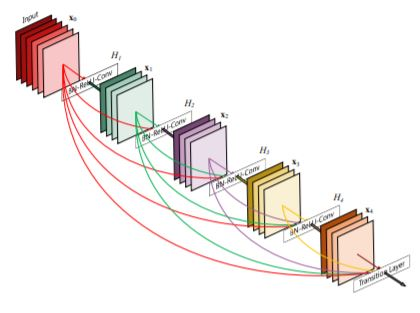
\includegraphics[width=.5\textwidth]{imagem/0x_densenet_block.jpg}
	% Caption centralizada
	\captionsetup{justification=centering}
	\captionfont{\small{\textbf{\\Fonte: \citeonline{liu-2017}.}}}	
	\label{fig:blocodenso}
\end{figure}

A Figura \ref{fig:blocodenso} mostra como se conectam as camadas na \ac{DenseNet}. Supondo que temos um bloco denso $B$ com um conjunto de 5 camadas $C = \{c_1, c_2, c_3, c_4, c_5\}$. Como explicado no parágrafo anterior, a saída das camadas serão utilizadas em todas as camadas subsequentes no mesmo bloco. Sendo assim, a entrada de $c_3$ será composta pelas saídas de $c_1$ e $c_2$ concatenadas, e assim sucessivamente. Além disso, como as saídas são concatenadas e não somadas, a tendência é que as entradas cresçam a medida que a rede se aprofunda. O conceito de bloco denso permite propagar múltiplos níveis de abstração ao longo de toda a rede, melhorando assim os resultados obtidos \cite{liu-2017}.

\citeauthor{liu-2017} ficaram em segundo lugar no \ac{ILSVRC} de 2017 e venceram o prêmio de melhor artigo da \ac{CVPR} do mesmo ano.

%%% p2 Escrever sobre os resultados obtidos pelas CNNs em Localização de Objetos
Nas tarefas de localização de objetos as \ac{CNN}s também têm se destacado com bons resultados. \citeonline{redmon-2015} propuseram o \ac{YOLO} e obtiveram um bom resultado fazendo localização e classificação de objetos em tempo real, conseguindo processar 45 \ac{FPS} com uma \ac{mAP} de 63,4\%. \citeonline{sren-2017} propuseram o \ac{R-CNN} e conseguiram obter resultados significativamente melhores para as tarefas de localização e classificação chegando a uma \ac{mAP} de até 78,8\%. Numa implementação alternativa com o enfoque no processamento em tempo real, a \ac{mAP} cai um pouco, chegando a 73,2\% porém, ele processa apenas 7 \ac{FPS}.

\citeonline{wei-2015} propuseram o \ac{SSD}, uma abordagem que além de obter uma \ac{mAP} elevada (74,3\%), supera a velocidade alcançada no \ac{YOLO} atingindo 59 \ac{FPS}. Esses resultados são especialmente relevantes, pois, além de serem competitivos com o estado da arte, trabalham com imagens menores - enquanto os quadros processados pelo \ac{YOLO} têm dimensões $448 \times 448$ e os processados pelo \ac{R-CNN} têm $1000\times 600$, o \ac{SSD} processa quadros de dimensões $300 \times 300$. O principal ganho em trabalhar com imagens menores é diminuir o consumo de memória e ter um método mais robusto por poder obter resultados competitivos mesmo que com imagens menores. Por um outro lado, trabalhar com imagens menores pode significar que o método seja mais lento ao processar imagens maiores.

%%% p3 Escrever sobre os resultados obtidos pelas CNNs em Segmentação semantica usando deconvolução
Uma outra área impactada pelo uso das \ac{CNN}s é a área de segmentação semântica. \citeonline{long-2014} propuseram o uso de uma \ac{FCN} para fazer segmentação semântica e conseguiram obter resultados superiores ao estado da arte, utilizando camadas de deconvolução para aumentar a resolução dos mapas de filtros gerados na saída da \ac{CNN}. \citeonline{noh:2015} propuseram um trabalho mais avançado de forma a tratar algumas limitações encontradas por \citeonline{long-2014}. Essa arquitetura funciona com a estrutura de um \textit{autoencoder}, usando as camadas de deconvolução que não servem para aumentar a resolução, mas para recuperar as informações da imagem de forma mais refinada, de forma a melhorar os resultados da segmentação.

%%% p4 Escrever sobre os resultados obtidos pela DSSD
Por fim, \citeonline{cheng-2017} propôs uma abordagem alternativa na resolução dos problemas de localização e classificação de objetos utilizando camadas de deconvolução a \ac{DSSD}. A \ac{DSSD} recebe essa sigla, pois é uma extensão do \ac{SSD} \cite{wei-2015}. A diferença é que, ao final, ele acrescenta camadas de deconvolução e, com os resultados das deconvoluções ele faz a classificação e a localização. Os resultados obtidos superam os apresentados pelo \ac{SSD} em \ac{mAP}, alcançando 81,5\% embora, o  \ac{DSSD} perde na velocidade (13,6 FPS). 

\section{Motivação}
\label{secao:1:1}

%%% p1 Mencionar como as CNNs tem sido objetos de estudo recentemente
Estudos envolvendo redes neurais convolucionais têm sido realizados com muita frequência tanto em áreas gerais, quanto aplicados à áreas específicas. Estudos vem sendo feitos para classificação de imagens \cite{krizhevsky-2012, simonyan-2014}, classificação e detecção de objetos \citeonline{cheng-2017, lin-2014}, segmentação de imagens \citeonline{long-2014, noh:2015}, segmentação de objetos em vídeos \citeonline{caelles-2017, voigtlaender-2017}. Isso se deve aos bons resultados obtidos pelos métodos aplicados nas respectivas áreas.

%%% p2 Mencionar como as aplicações dos algoritmos de detecção
Além disso, o problema de classificação e detecção de objetos tem sido aproveitado como solução para problemas mais específicos, como detecção facial \cite{yang-2018}, contagem de pessoas \cite{pren-2017} e detecção de pedestres \cite{lan-2018}. 

%%% p3 Mencionar a espectativa ao usar deconvolução
Por fim o uso de camadas adicionais de convolução ao final de uma \ac{CNN} pode gerar bons resultados na localização e classificação de objetos como apresentado por \citeonline{wei-2015} e \citeonline{cheng-2017}. Em suma, pode-se dizer que o tema ainda tem muito que ser explorado, que a proposta é promissora, e que bons resultados podem trazer contribuições para trabalhos futuros.

%Por fim o uso das camadas de deconvolução no método proposto traz boas expectativas, uma vez que já há resultados na literatura que mostram a sua eficiência \cite{noh:2015, cheng-2017}. Em suma, pode-se dizer que o tema ainda tem muito que ser explorado, que a proposta é promissora, e que bons resultados podem trazer contribuições para trabalhos futuros.

\section{Objetivos}
\label{secao:1:2}  

O objetivo do trabalho é utilizar a rede \ac{DenseNet}121 modificada com camadas adicionais de convolução %e deconvolução 
para fazer detecção e classificação de objetos. Para isso, será necessário:

\begin{itemize}
	\item Adaptar a \ac{CNN} \ac{DenseNet} \cite{liu-2017} para fazer localização e classificação de forma similar à \ac{SSD};
	%\item Alterar a arquitetura da rede inicial para receber camadas de deconvolução de forma a melhorar os resultados da classificação e da Localização;
	\item Avaliar os resultados obtidos comparando-os com a literatura.
\end{itemize}

\section{Justificativa}
\label{secao:1:3}

Com os avanços tecnológicos alcançados ao longo das últimas décadas, a produção de conteúdo multimídia tem crescido consideravelmente e tem sido amplamente explorada pelos mais diversos setores da sociedade. Todos os dias mais de 95 milhões de fotos e vídeos são postadas no Instagram\footnote{https://www.instagram.com}. Esse imenso volume de dados que são produzidos e acessados em multimídia inviabiliza a manipulação deste conteúdo por meio de ação humana; criando assim, a necessidade de automatizar a recuperação e análise de informações relevantes contidas nas mesmas.

Nesse sentido, todos os dias são estudados novos algoritmos e novas técnicas para fazer recuperação de informação multimídia. E uma das formas amplamente utilizadas é a de localização e classificação de objetos em imagens. \citeonline{everingham-2015} definem que o problema de classificação consiste em responder para cada classe de objeto se existe ou não uma ou mais instâncias daquele objeto na imagem e, o problema de localização consiste em dizer onde na imagem estão as instâncias dos objetos reconhecidos pelo classificador.

É válido estabelecer que ``os mecanismos sensitivos dos seres humanos (como visão e audição) sugerem a necessidade de uma arquitetura profunda para extrair a sua estrutura complexa'' \cite{deng-2014}. Porém, de acordo com \citeonline{caelles-2017}, uma grande limitação ao utilizar arquiteturas de \emph{Deep Learning} é a necessidade de treinamento com um grande volume de dados. Essa limitação torna o processo mais custoso em termos de tempo de processamento e outros recursos computacionais(como memória). Além disso, a base de dados deve ter os resultados da classificação e localização esperados feitos de forma manual, o que aumenta o esforço humano.

Tendo isso em vista, a proposta de utilizar a \ac{DenseNet} \cite{liu-2017} pré-treinada em classificação de imagens visa diminuir o custo por meio do \textit{Transfer Learning}. Além disso, utilizando as camadas adicionais de convolução como proposto por \citeonline{wei-2015}, espera-se obter resultados ainda melhores. Esses resultados melhores repercutiriam de forma positiva em outras áreas relacionadas à localização e classificação de objetos. 

\section{Organização do texto}
\label{secao:1:4}

O Capítulo \ref{cap:2} traz os principais conceitos relacionados à \textit{Deep Learning}, redes neurais artificiais, classificação de objetos em imagens e detecção de objetos em imagens, necessários à compreensão do trabalho. O Capítulo \ref{cap:3} contém um resumo dos trabalhos relacionados à monografia. O Capítulo \ref{cap:4} contém a metodologia a ser seguida para o desenvolvimento do trabalho. O Capítulo \ref{cap:5} descreve os experimentos realizados e os resultados obtidos. O Capítulo \ref{cap:6} apresenta a conclusão do trabalho com base nos resultados obtidos e apresenta propostas de trabalhos futuros.
% Os demais capítulos não precisam começar no anverso
\setboolean{@openright}{false}
% Nome do capítulo
\chapter{Revisão Bibliográfica}
\label{cap:2}
\vspace{-1.9cm}

Neste capítulo serão apresentados os principais conceitos e definições da literatura sobre \ac{RNA}, Deep Learning, classificação e localização de objetos.

\section{\textit{Machine Learning}}
\label{secao:2:1}
\vspace{-.6cm}

\textit{Machine Learning} ou Aprendizado de Máquina é um campo de estudo cada vez mais recorrente na área de tecnologia. Em uma definição alternativa, pode-se dizer que ``[...]Aprendizado de Máquina é uma área de Inteligência Artificial cujo objetivo é o desenvolvimento de técnicas computacionais sobre o aprendizado bem como a construção de sistemas capazes de adquirir conhecimento de forma automática.'' \cite{monard-2003}. Entre as principais aplicações de Aprendizado de máquina, pode se destacar o reconhecimento de padrões, classificação de imagens e a mineração de dados. 

\citeonline{monard-2003} definem ainda que o aprendizado de máquina pode ser supervisionado ou não-supervisionado. Quando falamos do primeiro caso, queremos dizer que o algoritmo recebe um conjunto de dados na entrada, processa esses dados e retorna uma saída. Essa saída é comparada com um valor previamente associado à entrada, comumente conhecido como rótulo. Já no aprendizado não-supervisionado, as entradas não possuem rótulo algum, cabendo ao algoritmo fazer a distinção das diversas entradas. Geralmente, nesses casos é necessária uma análise posterior à execução do algoritmo para se entender os resultados obtidos.

O aprendizado supervisionado se divide em dois grupos menores: classificação e regressão. \citeonline{santos-2012} define que quando o problema possui um conjunto discreto de saídas e o objetivo é atribuir a qual dessas saídas a entrada pertence, se trata de um problema de classificação. \citeonline{santos-2012} define ainda que quando o objetivo é prever uma saída de valor contínuo pra uma entrada, se trata de um problema de regressão.

As seções \ref{subsecao:2:1:1} e \ref{subsecao:2:1:2} irão definir melhor esses conceitos.

\subsection{Regressão}
\label{subsecao:2:1:1}

Como definido anteriormente, o problema de regressão consiste em calcular para cada entrada uma saída que possua um valor contínuo. \citeonline{dosualdo-2003} define que a regressão consiste em fazer uma relação entre os atributos $X={x_1, x_2,..., x_n}$ - onde $X$ é o conjunto de entrada e cada $x_i$ é um atributo numérico ou quantitativo - e $Y$, tal que $Y$ é um atributo ou um conjunto de atributos meta. \citeonline{apte-1997} definem essa relação por meio da Equação  \ref{eq:eq1}.

\begin{equation}
\label{eq:eq1}
	Y = f(x_1, x_2,..., x_n)
\end{equation}

A relação entre o(s) atributo(s) $X$ e o(s) atributo(s)-meta $Y$ alcançada como resultado de um algoritmo de regressão é chamado de modelo. Após a definição do modelo é importante fazer uma avaliação para dizer o quão confiável será a predição gerada pelo modelo. Existem diversas funções usadas na avaliação dos algoritmos de regressão, e uma das mais comuns é o \ac{MSE} que é definido pela Equação  \ref{eq:eq2}.

\begin{equation}
\label{eq:eq2}
	E = \dfrac{1}{N}\sum_{i = 0}^{N}(Y_i - f(X)_i)^2
\end{equation}

\noindent
Em que $E$ é o erro, $N$ é o tamanho do conjunto de amostras, $Y_i$ é o valor esperado do atributo-meta e $f(X_i)$ é o resultado do modelo para a entrada $X_i$. O objetivo do treinamento da predição, é minimizar esse erro quadrático, de forma que - em tese - o resultado previsto seja próximo do esperado.

Alguns exemplos de problemas de regressão são: 

\begin{enumerate}
	\item Predizer o percentual de gordura que uma pessoa possui no corpo, recebendo como entrada atributos como altura, idade, peso, sexo \cite{dosualdo-2003};
	\item Predizer o preço de um imóvel baseado em atributos como o tamanho, número de cômodos, número de quartos, etc. \cite{pereira-2012}.
\end{enumerate}

Uma grande limitação nos métodos de regressão é que eles em sua maioria solucionam problemas que possuem apenas um atributo-meta. Porém, os métodos de regressão baseados em \ac{RNA} podem retornar múltiplos resultados. Esse termo será definido na Sessão \ref{secao:2:2}.

\subsection{Classificação}
\label{subsecao:2:1:2}

Como mencionado anteriormente, o problema de classificação consiste em fazer uma predição quando as saídas são discretas. A ideia dos algoritmos de classificação é definir para cada entrada, um rótulo ou classe no meio de um conjunto finito de rótulos. Um método estatístico muito utilizado nos problemas de classificação é a regressão logística. A regressão logística é bem similar à regressão linear, com a diferença que o resultado é um número entre zero e um, configurando na verdade, a probabilidade de, dado uma entrada $X$ tal que $X = {x_1, x_2, ..., x_n}$ gerar uma saída verdadeira para a hipótese $Y$. Normalmente, os modelos de regressão logística aplicam a função sigmóide, descrita pela Equação  \ref{eq:eq3}.

\begin{equation}
\label{eq:eq3}
Y = \dfrac{1}{1 + e^{-g(X)}}
\end{equation}

A regressão logística se ajusta muito bem a problemas de classificação binária. Porém, a grande maioria dos problemas de classificação possuem mais de uma classe, consistindo então em dizer para uma entrada $X$ tal que $X = [x_1, x_2, ..., x_n]$ a qual classe de $Y$ ela pertence, tal que $Y = [y_1, y_2, ..., y_m]$. \citeonline{Thanh-2015} afirmam que as principais abordagens para solucionar problemas de classificação com $M$ classes consistem em dividir o problema em vários problemas de classificação binária.

Essa divisão pode ser feita de duas formas diferentes: 
\begin{itemize}
	\item A primeira consiste em gerar $M - 1$ problemas de classificação binária e resolver cada um de forma independente. Após resolver os problemas de classificação, determinar a classe final a partir das probabilidades obtidas selecionando a classe que obteve a maior probabilidade. Essa abordagem é conhecida como \textit{one-versus-all}.
	\item A segunda consiste em combinar as classes em pares e, para cada par de classe gerar um problema de classificação. Isto é, seja $Y$ um conjunto de classes, para cada classe $y \in Y$ criar um problema de classificação para $y$ e  cada $y_\beta$ tal que $y_\beta \in Y - [y]$. Isso gera um conjunto de $\frac{M (M - 1)}{2}$ problemas de classificação. Após gerar e solucionar os problemas, o resultado será a classe que for mais vezes selecionada.
\end{itemize}

Com base na primeira abordagem, começou a ser utilizada uma função para os problemas de classificação que envolvem múltiplas classes. Essa função é a \textit{softmax} que calcula o valor de cada saída e divide pela soma das saídas, gerando assim uma saída normalizada que corresponde à probabilidade de o dado de entrada estar na classe. Atualmente é a função mais utilizada para problemas de classificação com múltiplas classes e é descrita pela Equação  \ref{eq:eq4}.

\begin{equation}
\label{eq:eq4}
	f(x)_i = \dfrac{e^{\beta x_i}}{\sum_{j = 1}^{K}e^{\beta x_j}} \forall i = 1,...,K e x = {x_1, ... ,x_k} \in X^K
\end{equation}

Assim como na regressão linear, a perda na regressão logística pode ser calculado pelo \ac{MSE}. Porém, com o tempo, surgiram outras funções que calculam a perda de forma mais eficiente em problemas de classificação.

\section{Redes Neurais Artificiais}
\label{secao:2:2}

As \ac{RNA}s são uma das principais técnicas de aprendizagem de máquina e podem ser implementadas tanto para problemas supervisionados, quanto não-supervisionados. \citeonline{jost-2015} definiu as \ac{RNA}s da seguinte forma:

\begin{citacao}
	As \ac{RNA}s possuem inspiração nas redes neurais biológicas, constituídas de neurônios separados por camadas, que processam informações e estão conectados via pesos sinápticos, sendo na maioria das vezes sistemas adaptativos que modificam sua estrutura através de informações, que fluem pela rede durante a etapa de aprendizado \cite{jost-2015}.
\end{citacao}

Além disso, é importante mencionar que em uma rede neural, existem duas camadas em particular que são muito importantes: a primeira camada, que é a camada de entrada de dados, e a última camada que é a camada de saída. Existem dois tipos de \ac{RNA}s: as redes \textit{feed forward}, que processa apenas o estado atual das entradas, e as redes neurais recorrentes que processa o estado atual e o estado anterior. As redes neurais recorrentes podem ser usadas de forma eficiente para processar vídeos, séries temporais e outros dados que possuam múltiplos estados.

A \ac{RNA} \textit{feed forward} mais básica que existe é a \textit{Perceptron}, composta apenas por um conjunto de neurônios de entrada e um único neurônio de saída. A Equação  \ref{eq:eq5} representa a fórmula de um \textit{Perceptron}, onde $n$ é o número de entradas, $W_i$ são os respectivos pesos de cada entrada, $X_i$ são as entradas e $B$ é o viés do neurônio.

\begin{equation}
Y=\Big(\sum_{i=1}^{n}{(W_i \times X_i)}\Big) - B
\label{eq:eq5}
\end{equation}

Uma rede percepron não é uma arquitetura de redes neurais artificiais muito poderosa, mas deu base para outras arquiteturas mais robustas. A principal delas é o \textit{Perceptron} Multi-Camadas.

\subsection{\textit{Multi-Layer Perceptron}}
\label{subsecao:2:2:2}


As redes \textit{Perceptron} Multicamadas ou \ac{MLP} são baseadas nos \textit{Perceptron}s simples, como mencionado anteriormente. A diferença, porém, é que elas trabalham com mais camadas do que simplesmente as camadas de entrada e saída. Geralmente elas possuem uma ou duas camadas intermediárias às camadas externas. Essas camadas intermediárias, também são chamadas de camadas ocultas e servem para conferir uma robustez maior ao método.

Nas \ac{MLP}s, uma outra diferença é que as funções de ativação podem variar. As mais comuns são o \ac{ReLU} (definido pela Equação  \ref{eq:eq6}), a função sigmóide (descrita na Seção \ref{subsecao:2:1:2}) e a tangente hiperbólica (definida pela Equação  \ref{eq:eq7}).

\begin{equation}
	Y(x) = max(0, x)
	\label{eq:eq6}
\end{equation}

\begin{equation}
	Y(x) = \dfrac{e^x - e^{-x}}{e^x+e^{-x}}
	\label{eq:eq7}
\end{equation}

Como foi dito anteriormente, a \ac{MLP} trabalha com aprendizado supervisionado, isso quer dizer que os dados que ela opera são rotulados, e tem uma saída esperada. Quando as entradas são processadas e os resultados das saídas são calculados, eles são comparados com os valores esperados pelos rótulos e é gerado a função de erro quadrático, definida na Seção \ref{subsecao:2:1:1}.

Sabendo-se disso, o objetivo para melhorar a precisão da \ac{MLP} é minimizar o valor da função erro, ou seja, tornar as saídas da rede o mais próximo possível das saídas esperadas. Para tanto, é utilizado o método de retropropagação de erro que reajusta os pesos da rede de acordo com os valores obtidos usando a descida de gradiente.

\citeonline{arnold-2011} definem que aumentar o número de camadas em um \ac{MLP} não garante uma melhoria dos resultados, pois a descida de gradiente pode chegar a um mínimo local. Além disso, o aumento do número de camadas implica em um tempo muito maior de processamento. Para lidar com esse problema surge o \emph{Deep Learning}, uma arquitetura avançada com múltiplas camadas, que soluciona a dificuldade que as redes neurais possuem ao lidar com dados de alta dimensionalidade \cite{arnold-2011}.

\section{\textit{Deep Learning}}
\label{secao:2:3}

A principio não parecia ser viável manipular arquiteturas profundas de redes neurais. Porém, de acordo com \citeonline{deng-2014}, surgiu um algoritmo de aprendizado não-supervisionado que conseguiu aliviar empiricamente as dificuldades de otimização em arquiteturas profundas. Esse algoritmo é a \ac{DBN}, um modelo generativo profundo composto de uma camada visível e várias camadas ocultas compostas por uma pilha de \ac{RBM}s.

\citeonline{deng-2014} definem ainda que o aprendizado nas \ac{DBN}s é feito por um algoritmo guloso que ajusta os pesos camada-por-camada com uma complexidade linear ao tamanho e à profundidade da rede. E uma relação inesperada entre as \ac{DBN}s e as \ac{MLP}s surgiu quando descobriu-se que ao utilizar os pesos de uma \ac{DBN} com arquitetura correspondente, você consegue inicializar os pesos de uma \ac{MLP} de forma a produzir melhores resultados do que utilizando pesos aleatórios.

Uma segunda alternativa para trabalhar com aumento de camadas é o empilhamento de auto-codificadores. O empilhamento de auto-codificadores consiste basicamente em inserir na saída de uma rede neural uma segunda rede neural que para cada entrada produz uma saída específica e retreinar a nova rede neural utilizando o algoritmo de retropropagação de erro \cite{deng-2014}.

\subsection{Redes Neurais Convolucionais}
\label{subsecao:2:3:1}

As \ac{CNN} são um modelo específico de \textit{Deep Learning} muito utilizados em aplicações de visão computacional e aplicações de reconhecimento de imagens. De acordo com \citeonline{ferreira-2017}, as \ac{CNN}s utilizam matrizes para processar as entradas de dados, sendo essas matrizes unidimensionais para sinais e sequências, bidimensionais para imagens e tridimensionais para imagens volumétricas e vídeos. 

Ao contrário das \ac{RNA}s tradicionais (como \ac{MLP}), as \ac{CNN}s não necessariamente ligam todos os neurônios na camada de origem a todos os neurônios da camada de destino. \citeonline{ferreira-2017} define que existem três tipos comuns de camadas utilizadas nas redes neurais convolucionais: as camadas de convolução, camadas de \textit{pooling} e camadas completamente conexas.

A ideia da camada de convolução é de que cada neurônio recebe como entrada neurônios próximos e tem por objetivo criar mapas e filtros. \citeonline{ferreira-2017} define que em aplicações de reconhecimento de objetos, por exemplo, é comum as primeiras camadas de convolução detectarem bordas ou manchas que seriam as características mais básicas da imagem. As camadas de convolução mais profundas detectam outras características mais específicas.

As camadas de \textit{pooling} são utilizadas para reduzir a dimensão de dados vindo das camadas de convolução, consequentemente reduzindo o custo computacional \cite{ferreira-2017}. Na prática elas funcionam como as camadas de convolução, mas ao invés de fazer a operação tradicional de convolução, elas reduzem um conjunto de elementos a um único representante com base em uma função específica. As funções mais utilizadas são máximo e média \cite{ferreira-2017}.

Por fim, as camadas completamente conexas são exatamente iguais às redes MLP e é comum utilizá-las no final da rede para conectar à saída. Seu acréscimo no final é importante pois faz a ligação de todos os filtros \cite{ferreira-2017}. As arquiteturas de \ac{CNN}s geralmente intercalam algumas camadas de convolução com uma camada de \textit{pooling}. As arquiteturas mais antigas costumavam adicionar camadas completamente conexas ao final, porém, os modelos mais novos, como a \ac{ResNet} e a \ac{DenseNet} já não usam mais esse conceito.


%%%%%%%%%%%%%%%%%%% Formato para a inserção de figuras

%  \begin{figure}[H]
  % Alterar espaçamentos antes e depois do caption
%  \setlength{\abovecaptionskip}{0pt}
%  \setlength{\belowcaptionskip}{0pt}
  % Caption
%  \caption[Principais componentes de WiNoCs]{Principais componentes de WiNoCs}
%  \centering
%  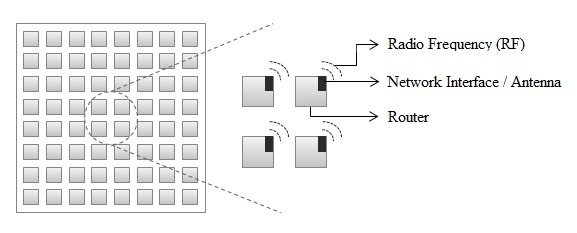
\includegraphics[width=.85\textwidth]{imagem/winoc.jpg}
  % Caption centralizada
%  \captionsetup{justification=centering}
%  \captionfont{\small{\textbf{\\Fonte: \cite{OliveiraIadis:2011}}}}	
%  \label{fig:ComponentesWiNoC}
%  \end{figure}


%%%%%%%%%%%%%%%%%%%%%%%%%% Modelo para inserir gráficos

%\begin{grafico}[H]
  % Alterar espaçamentos antes e depois do caption
%  \setlength{\abovecaptionskip}{5pt}
%  \setlength{\belowcaptionskip}{0pt}
  % Caption
%  \caption[Percentual de pacotes enviados]
%	  {Percentual de pacotes enviados}
%  \centering
%  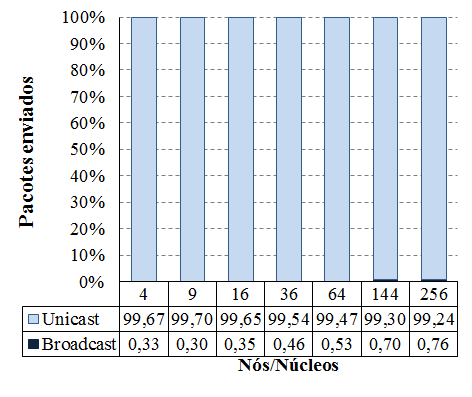
\includegraphics[width=.48\textwidth]{imagem/graficos/grafico_pacotes_enviados_bt.png}
  % Caption centralizada
%  \captionsetup[grafico]{justification=centering}
  % Fonte
%  \captionfont{\small{\textbf{\\Fonte: Dados da pesquisa}}}
%  \end{grafico}


%\begin{grafico}[H]
  % Alterar espaçamentos antes e depois do caption
%  \setlength{\abovecaptionskip}{5pt}
%  \setlength{\belowcaptionskip}{0pt}
  % Caption
%  \caption[Resultados da carga de trabalho 1]
%	  {Resultados da carga de trabalho 1}
%  \centering
%  \subfloat[Enviados]
%      {\label{graf:enviados_bt}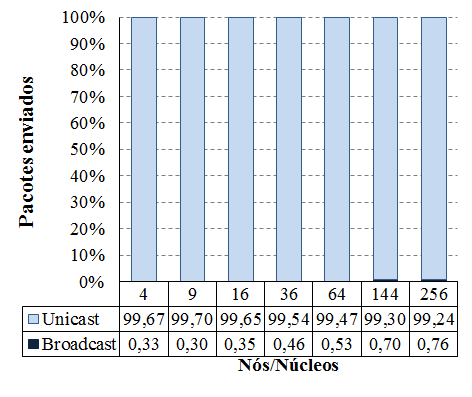
\includegraphics[width=.48\textwidth]{imagem/graficos/grafico_pacotes_enviados_bt.png}} \quad
%  \subfloat[Perdidos]
%      {\label{graf:perdidos_bt}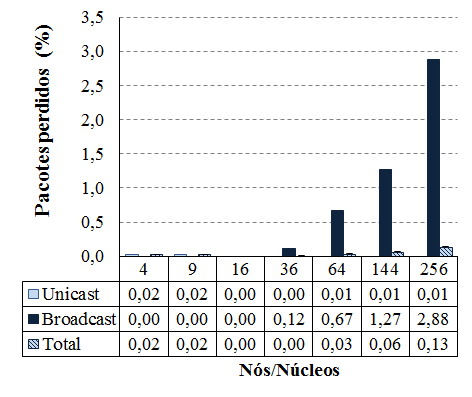
\includegraphics[width=.48\textwidth]{imagem/graficos/grafico_pacotes_perdidos_bt.png}} \quad
%  \subfloat[Taxa de injeção]
%      {\label{graf:injecao_bt}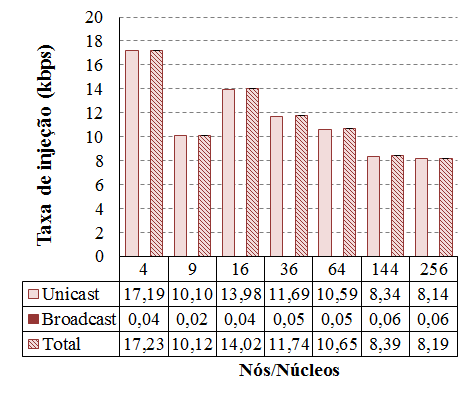
\includegraphics[width=.48\textwidth]{imagem/graficos/grafico_taxa_injecao_bt.png}} \quad
%  \subfloat[Vazão]
%      {\label{graf:vazao_bt}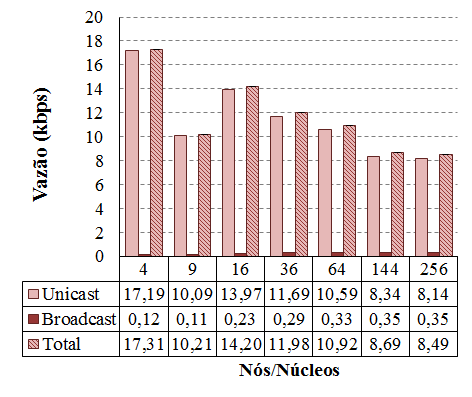
\includegraphics[width=.48\textwidth]{imagem/graficos/grafico_vazao_bt.png}}
  % Caption centralizada
%  \captionsetup[grafico]{justification=centering}
  % Fonte
%  \captionfont{\small{\textbf{\\Fonte: Dados da pesquisa}}}
%  \label{graf:quad}
%  \end{grafico}

%%%%%%%%%%%%%%%%%%%%%%%% Exemplo de criação de tabelas

   % Tabela
%  \begin{table}[H]
%    \centering
%    \footnotesize
    % Alterar espaçamentos antes e depois do caption
%    \setlength{\abovecaptionskip}{0pt}
%    \setlength{\belowcaptionskip}{0pt}
    % Caption
%    \caption[Parâmetros definidos por classe]{Parâmetros definidos por classe}
%    \label{tab:classesNas}
    % Conteúdo da tabela
%    \begin{tabular}{c|c|c|c|c|c|c|c}
%	\hline \hline
%	\textit{Benchmark} &	Parâmetro &	Classe S &	Classe W &	Classe A &	Classe B &	Classe C &	Classe D \\ 
%	\hline \hline
% 	BT & \textit{Grid}	& $12^3$	& $24^3$ 	& $64^3$	& $102^3$ 	& $162^3$	& $408^3$ \\ 
%	CG & Linhas		& 1400		& 7000 		& 14000 	& 75000 	& 150000 	& 1500000 \\ 
%	EP & Pares 		& $2^{24}$	& $2^{25}$	& $2^{28}$	& $2^{30}$	& $2^{32}$	& $2^{36}$ \\
%	FT & \textit{Grid}	& $64^3$	& $128^2*32$	& $256^2*128$	& $512*256^2$	& $512^3$	& $2048*1024^2$ \\ 
%	IS & Chaves		& $2^{16}$	& $2^{20}$	& $2^{23}$	& $2^{25}$	& $2^{27}$	& $2^{31}$ \\ 
%	LU & \textit{Grid}	& $12^3$	& $33^3$	& $64^3$	& $102^3$	& $162^3$	& $408^3$ \\
%	MG & \textit{Grid}	& $32^3$	& $128^3$	& $256^3$	& $256^3$	& $512^3$	& $1024^3$ \\ 
%	SP & \textit{Grid}	& $12^3$	& $36^3$	& $64^3$	& $102^3$	& $162^3$	& $408^3$ \\
%	\hline \hline
%    \end{tabular}
    % Fonte
%    \captionfont{\small{\textbf{\\Fonte: Adaptado de \cite{Nas:2011}}}}
%  \end{table}
% Nome do capítulo
\chapter{Trabalhos Relacionados}
\label{cap:3}
\vspace{-1.9cm}

Neste capítulo serão apresentados os trabalhos na literatura que possuem relação com o trabalho proposto.

\section{DenseNet}
\label{secao:3:1}

Como mencionado anteriormente, desde 2012 as tarefas de classificação de imagens são resolvidas majoritariamente por arquiteturas de \textit{Deep Learning}. \citeonline{he-2016} propuseram uma nova arquitetura que utilizava o conceito de \textit{skip connection}, que, como explicado anteriormente, consiste em utilizar a saída de uma camada em camadas posteriores além da próxima. O conceito de \textit{skip connection} fez tanto sucesso que tornou a ser utilizado em um modelo mais recente. \citeonline{liu-2017} propuseram um modelo de \ac{CNN} que utiliza esse mesmo conceito, porém de uma forma um pouco diferente. 

Nas \ac{ResNet}s, existem os blocos residuais, conforme a Figura \ref{fig:blocoresidual}. No bloco residual temos duas camadas $c_1$ e $c_2$ onde $c_1$ é a entrada de $c_2$. Na saída deste bloco residual será feita uma soma de matrizes entre a saída de $c_2$ e a entrada de $c_1$ e essa soma será usada na entrada das camadas posteriores. 

Nas \ac{DenseNet}s, o conceito de \textit{skip connection} é utilizado conforme a Figura \ref{fig:blocodenso}. Um bloco denso $B$ composto por um conjunto de camadas $C = \{c_1, c_2, ..., c_n\}$ onde $c_1$ é a entrada de $c_2$. A primeira diferença é que para as camadas sucessoras, todas as camadas anteriores estarão na entrada, isso é, a entrada de $c_3$ será $\{c_1, c_2\}$, a entrada de $c_4$ será $\{c_1, c_2,c_3\}$ e assim sucessivamente. A segunda diferença é que nos blocos densos as saídas das camadas são unidas por uma concatenação de matrizes, não por soma. Sendo assim, se cada camada do bloco possui uma saída de $x$ matrizes, o bloco possui $n$ camadas e a entrada do bloco possui tamanho $a$, a saída possuirá o tamanho representado pela Equação~\ref{eq:eq8}:

\begin{equation}
	\label{eq:eq8}	y = n x + a
\end{equation}

Vale mencionar que o valor de $x$ se conserva para toda a rede. Uma vantagem de usar blocos densos é a possibilidade de propagar informações com diversos níveis de abstração ao longo de toda a rede.

As \ac{DenseNet}s seguem um padrão arquitetural muito similar ao das \ac{ResNet}s começando a rede com uma camada de convolução $7\times7$ com \textit{strides} de $2\times2$ que é sucedida por uma camada de \textit{batch normalization} e outra de \ac{ReLU}. Depois disso, têm uma camada de \textit{pooling} pelo máximo e após essa camada, têm quatro blocos densos intercalados por blocos intermediários. Os blocos de convolução dentro dos blocos densos são compostos por uma camada de convolução $1\times1$ (que \citeonline{liu-2017} definem como camada de ``gargalo'') e uma camada de convolução $3\times3$. Vale mencionar que todas as camadas de convolução nos blocos densos são precedidas por uma camada de \textit{batch normalization} e \ac{ReLU}. Os blocos intermediários são compostos por uma camada de convolução $1\times1$ seguida de uma camada de \textit{pooling} pela média (que também é precedida por \textit{batch normalization} e \ac{ReLU}). No final dos 4 blocos densos, a rede possui mais uma camada de \textit{batch normalization} e \ac{ReLU} seguida por um \textit{pooling} pela média global e uma camada completamente conectada que faz a classificação. A Figura \ref{fig:archdensenet} mostra como é a arquitetura da rede.

\begin{figure}[H]
	% Alterar espaçamentos antes e depois do caption
	\setlength{\abovecaptionskip}{0pt}
	\setlength{\belowcaptionskip}{0pt}
	% Caption
	\caption[Arquitetura DenseNet]{Arquitetura DenseNet}
	\centering
	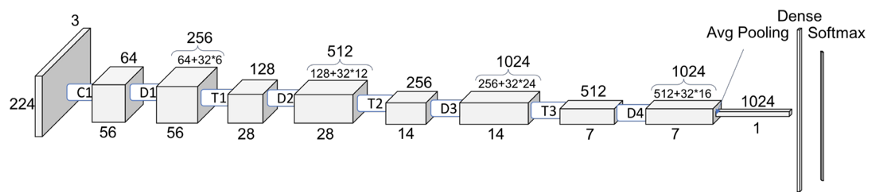
\includegraphics[width=.7\textwidth]{imagem/0x_densenet_arch.png}
	% Caption centralizada
	\captionsetup{justification=centering}
	\captionfont{\small{\textbf{\\Fonte: \citeonline{liu-2017}.}}}	
	\label{fig:archdensenet}
\end{figure}

O modelo proposto obteve resultados competitivos com os da literatura, ficando em segundo lugar no \ac{ILSVRC} de 2017 e apresentando resultados competitivos com os da literatura na época. O artigo também foi premiado como a melhor publicação da \ac{CVPR} do ano de 2017. O modelo obteve uma acurácia de 96\% na Cifar-10 e 82\% na Cifar-100.

\section{SSD: \textit{Single-Shot Multibox Detector}}
\label{secao:3:2}

\citeonline{wei-2015} propuseram um método a base de redes neurais convolucionais para fazer a localização e detecção de objetos. A proposta deles melhorou significativamente os resultados apresentados no estado da arte. Isso se deve ao fato de que eles não só conseguiram propor um modelo que faz a localização e classificação de forma eficiente (chegando a 74,3\% de \ac{mAP}), como conseguiram obter esse resultado fazendo classificação e localização em tempo real, com uma velocidade de 59 \ac{FPS}. Uma outra vantagem obtida por esse método é que ele consegue fazer a localização e classificação em imagens significativamente menores, uma vez que os quadros processados pelo \ac{YOLO} têm dimensões $448 \times 448$ e os processados pelo \ac{R-CNN} têm $1000\times 600$, o \ac{SSD} processa quadros de dimensões $300 \times 300$. Isso é uma vantagem, pois mesmo o algoritmo trabalhando com imagens menores, o resultado consegue competir com os outros métodos.

A abordagem consiste em utilizar a rede VGG16 \cite{simonyan-2014} como arquitetura base, substituir as camadas completamente conectadas fc6 e fc7 por camadas convolucionais, alterar o filtro pool5 de $2 \times 2 - s2$ para $3 \times 3 - s1$, e usaram o algoritmo \textit{à trous}\cite{holschneider-1990} para preencher os espaços vazios. Além disso, eles removeram todas as camadas de \textit{dropout} e a última camada completamente conectada. Por fim, as camadas de convolução geram os resultados de mais de 8000 localizações e classificações, as quais são filtradas em um passo final de supressão de não-máximos, que elimina todos os resultados com confiança abaixo de $0,5$.

A Figura \ref{fig:yoloxssd} mostra as diferenças entre as arquiteturas \ac{YOLO} e \ac{SSD}. Enquanto \citeonline{redmon-2015} usaram uma camada completamente conectada intermediária para fazer a localização dos objetos, \citeonline{wei-2015} usaram camadas de convolução sobre mapas de múltiplos tamanhos. Além disso, o \ac{SSD} trabalha com \textit{bounding-boxes} de tamanhos padrões $\{1, 2, 3, \frac{1}{2}, \frac{1}{3}\}$. Os filtros de convolução adicionais, os tamanhos padrões de \textit{bounding-boxes} e o uso de \textit{data-augmentation} foram cruciais na obtenção dos bons resultados.

  \begin{figure}[H]
	% Alterar espaçamentos antes e depois do caption
	\setlength{\abovecaptionskip}{0pt}
	\setlength{\belowcaptionskip}{0pt}
	% Caption
	\caption[YOLO e SSD]{Comparação entre \ac{YOLO} e \ac{SSD}}
	\centering
	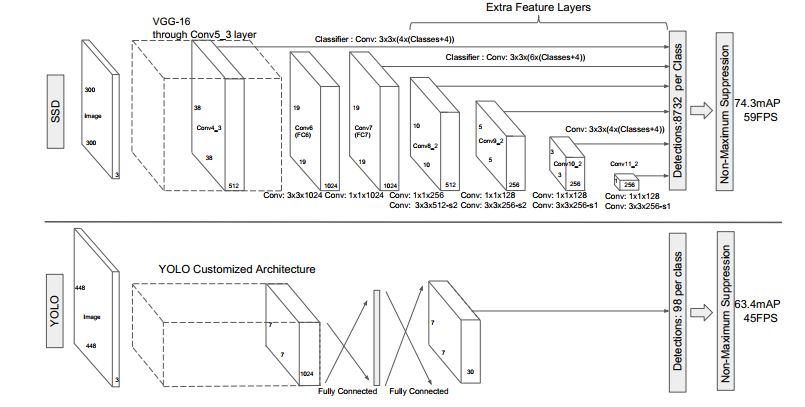
\includegraphics[width=.6\textwidth]{imagem/0x_yoloxssd.JPG}
	% Caption centralizada
	\captionsetup{justification=centering}
	\captionfont{\small{\textbf{\\Fonte: \citeonline{wei-2015}.}}}	
	\label{fig:yoloxssd}
\end{figure}

\section{DSSD: \textit{Deconvolution Single-Shot Detector}}
\label{secao:3:3}

\citeonline{cheng-2017} propuseram uma extensão do \ac{SSD}. Depois dos resultados obtidos pelo \ac{SSD} ao fazer localização e classificação de objetos com uma \ac{mAP} de $79,5\%$, eles propuseram uma abordagem alternativa, usando camadas de deconvolução ao final da rede. As camadas de deconvolução tem entre seus resultados o aumento de resolução do mapa de entrada. A abordagem visou explorar esse efeito com o intuito de aumentar a \ac{mAP} da classificação e localização de objetos, e, com isso, atingir uma \ac{mAP} de $81,5\%$. Embora essa abordagem tenha uma \ac{mAP} maior do que a obtida por \citeonline{wei-2015}, ela não é rápida o bastante pra fazer localização e classificação em tempo real.

A Figura \ref{fig:ssdxdssd} mostra as arquiteturas da \ac{SSD} e \ac{DSSD} mostrando as suas diferenças. É possível visualizar que a rede \ac{DSSD} utiliza as saídas da \ac{SSD} como entrada aos módulos de deconvolução.


\begin{figure}[H]
	% Alterar espaçamentos antes e depois do caption
	\setlength{\abovecaptionskip}{0pt}
	\setlength{\belowcaptionskip}{0pt}
	% Caption
	\caption[SSD e DSSD]{Comparação entre \ac{SSD} e \ac{DSSD}}
	\centering
	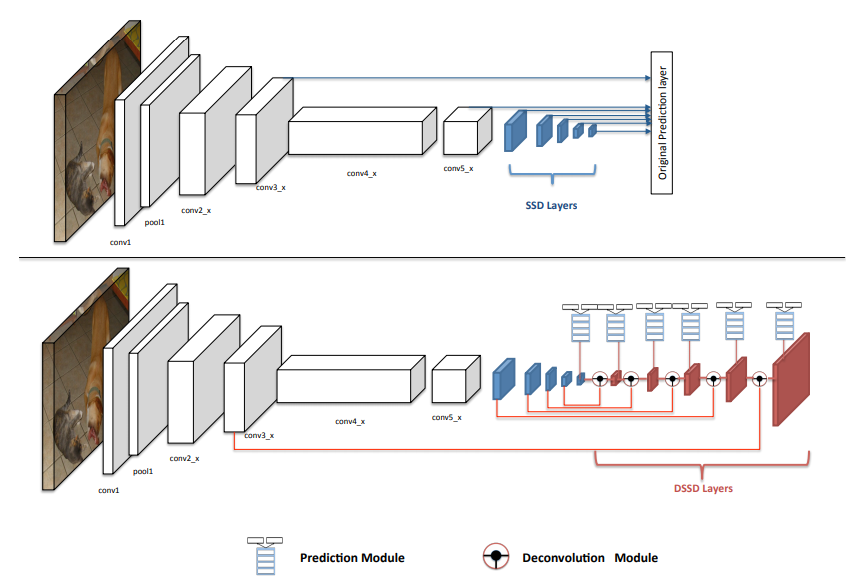
\includegraphics[width=.8\textwidth]{imagem/0x_comparacao_ssd_dssd.png}
	% Caption centralizada
	\captionsetup{justification=centering}
	\captionfont{\small{\textbf{\\Fonte: \citeonline{cheng-2017}.}}}	
	\label{fig:ssdxdssd}
\end{figure}

%Rever essa parte
Nesse trabalho, foram propostas duas alterações principais no modelo \ac{SSD}. A primeira delas foi a utilização da rede neural ResNet-101 \cite{he-2016}. \citeonline{cheng-2017} perceberam, porém, que apenas substituir a VGG16 pela \ac{ResNet} não produziria resultados melhores. Sendo assim, após adicionar as camadas de convolução do \ac{SSD} para fazer a detecção em múltiplos níveis, ele adicionou um módulo com mais algumas camadas de convolução a fim de melhorar os resultados. Os módulos propostos estão na Figura \ref{fig:ssdpred}.

\begin{figure}[H]
	% Alterar espaçamentos antes e depois do caption
	\setlength{\abovecaptionskip}{0pt}
	\setlength{\belowcaptionskip}{0pt}
	% Caption
	\caption[Módulos de predição SSD com ResNet]{Módulos de predição \ac{SSD} com \ac{ResNet}}
	\centering
	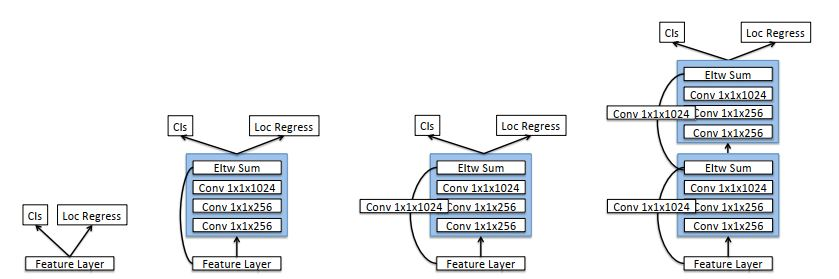
\includegraphics[width=.8\textwidth]{imagem/0x_dssdpredmod.jpg}
	% Caption centralizada
	\captionsetup{justification=centering}
	\captionfont{\small{\textbf{\\Fonte: \citeonline{cheng-2017}.}}}	
	\label{fig:ssdpred}
\end{figure}

Fazendo os testes, \citeonline{cheng-2017} perceberam que os melhores resultados foram obtidos usando a terceira opção que consistem um módulo residual com uma convolução na conexão alternativa e a junção das duas entradas sendo feita por meio de uma multiplicação elemento por elemento. Neste ponto, as mudanças ainda se mostravam pouco efetivas, já que a nova \ac{SSD}321 apresentava 77,1\% de \ac{mAP} contra 77,5\% de \ac{mAP} da \ac{SSD}300, ao passo que a nova \ac{SSD}513 apresentava 80,6\% contra 79,5\% da \ac{SSD}512.

Tendo isso em vista, após a implementação dos módulos \ac{SSD} na \ac{ResNet}101, \citeonline{cheng-2017} decidiram adicionar módulos usando camadas de deconvolução com o intuito de fazer um \textit{upsample} nas saídas da \ac{SSD} para obter mais dados. Depois de adicionar esses módulos, eles são combinados com o módulo \ac{SSD} anterior para gerar a nova saída. A Figura \ref{fig:deconv} mostra como é feita essa combinação.

\begin{figure}[H]
	% Alterar espaçamentos antes e depois do caption
	\setlength{\abovecaptionskip}{0pt}
	\setlength{\belowcaptionskip}{0pt}
	% Caption
	\caption[Módulos de deconvolução]{Módulos de deconvolução}
	\centering
	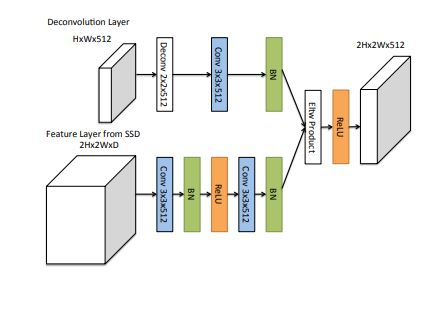
\includegraphics[width=.6\textwidth]{imagem/0x_dssd-deconv.jpg}
	% Caption centralizada
	\captionsetup{justification=centering}
	\captionfont{\small{\textbf{\\Fonte: \citeonline{cheng-2017}.}}}	
	\label{fig:deconv}
\end{figure}

Como mencionado anteriormente, embora o \ac{DSSD} tenha melhorado a \ac{mAP} do \ac{SSD}, ele não é aplicável para fazer a localização e classificação em tempo real. Com uma \ac{mAP} de $81,5\%$ ele consegue processar apenas $6,6$ \ac{FPS}. Isso se deve ao uso das deconvoluções, da ResNet 101 - que possui mais camadas, e, portanto toma mais tempo de processamento - e também ao aumento no número de \textit{bounding boxes} geradas($43688$ vs. $17080$), fazendo assim com que a supressão de não-máximos leve mais tempo.

\section{PASCAL VOC}
\label{secao:3:4}

Um grande desafio em treinar modelos de \textit{Deep Learning} é a necessidade de um grande volume de dados classificados manualmente. Com essa necessidade, diversos trabalhos foram desenvolvidos com o objetivo de apresentar uma base de dados anotados manualmente para um conjunto de problemas específicos. Nos trabalhos de Localização e classificação, uma das bases mais utilizadas é a \ac{PASCAL VOC}.

O desafio \ac{PASCAL VOC} foi realizado anualmente entre 2004 e 2012, e a cada ano novas imagens e novos desafios foram propostos na área de visão computacional. Os principais desafios envolviam Localização e Classificação de Objetos, Segmentação Semântica, \textit{layout} humano (um desafio que consiste em detectar partes do corpo como cabeça, mãos e pés) e classificação de ações \cite{everingham-2015}.

O desafio de Localização e Classificação de objetos desde 2007 possui 20 classes distintas de objetos e a cada ano eles criaram uma nova base com mais imagens extraídas da internet. A Tabela \ref{tab:voc2007} mostra as classes, o número de imagens e o número de objetos por classe nos conjuntos de treino, validação e teste.

\begin{table}[H]
	\centering
	\footnotesize
	% Alterar espaçamentos antes e depois do caption
	\setlength{\abovecaptionskip}{0pt}
	\setlength{\belowcaptionskip}{0pt}
	% Caption
	\caption[Pascal VOC 2007]{Classes de imagens do PASCAL VOC 2007}
	\label{tab:voc2007}
	\begin{tabular}{l|l|l|l|l|l|l|ll}
		& \multicolumn{2}{l|}{Treino} & \multicolumn{2}{l|}{Validação} & \multicolumn{2}{l|}{Treino/Validação} & \multicolumn{2}{l}{Teste}              \\ \hline
		& imagens      & Objetos      & Imagens        & Objetos       & Imagens           & Objetos           & \multicolumn{1}{l|}{Imagens} & Objetos \\ \hline
		Avião          & 112          & 151          & 126            & 155           & 238               & 306               & \multicolumn{1}{l|}{204}     & 285     \\
		Bicicleta      & 116          & 176          & 127            & 177           & 243               & 353               & \multicolumn{1}{l|}{239}     & 282     \\
		Pássaro        & 180          & 243          & 150            & 243           & 330               & 486               & \multicolumn{1}{l|}{282}     & 459     \\
		Barco          & 81           & 140          & 100            & 150           & 181               & 290               & \multicolumn{1}{l|}{172}     & 263     \\
		Garrafa        & 139          & 253          & 105            & 252           & 244               & 505               & \multicolumn{1}{l|}{212}     & 469     \\
		Ônibus         & 97           & 115          & 89             & 114           & 186               & 229               & \multicolumn{1}{l|}{174}     & 213     \\
		Carro          & 376          & 625          & 337            & 625           & 713               & 1250              & \multicolumn{1}{l|}{721}     & 1201    \\
		Gato           & 163          & 186          & 174            & 190           & 337               & 376               & \multicolumn{1}{l|}{322}     & 358     \\
		Cadeira        & 224          & 400          & 221            & 398           & 445               & 798               & \multicolumn{1}{l|}{417}     & 756     \\
		Vaca           & 69           & 136          & 72             & 123           & 141               & 259               & \multicolumn{1}{l|}{127}     & 244     \\
		Mesa de Jantar & 97           & 103          & 103            & 112           & 200               & 215               & \multicolumn{1}{l|}{190}     & 206     \\
		Cão            & 203          & 253          & 218            & 257           & 421               & 510               & \multicolumn{1}{l|}{418}     & 489     \\
		Cavalo         & 139          & 182          & 148            & 180           & 287               & 362               & \multicolumn{1}{l|}{274}     & 348     \\
		Motocicleta    & 120          & 167          & 125            & 172           & 245               & 339               & \multicolumn{1}{l|}{222}     & 325     \\
		Pessoa         & 1025         & 2358         & 983            & 2332          & 2008              & 4690              & \multicolumn{1}{l|}{2007}    & 4528    \\
		Vaso de planta & 133          & 248          & 112            & 266           & 245               & 514               & \multicolumn{1}{l|}{224}     & 480     \\
		Ovelha         & 48           & 130          & 48             & 127           & 96                & 257               & \multicolumn{1}{l|}{97}      & 242     \\
		Sofá           & 111          & 124          & 118            & 124           & 229               & 248               & \multicolumn{1}{l|}{223}     & 239     \\
		Trem           & 127          & 145          & 134            & 152           & 261               & 297               & \multicolumn{1}{l|}{259}     & 282     \\
		Monitor/TV     & 128          & 166          & 128            & 158           & 256               & 324               & \multicolumn{1}{l|}{299}     & 308     \\
		Total          & 2501         & 6301         & 2510           & 6307          & 5011              & 12608             & \multicolumn{1}{l|}{4952}    & 12032  
	\end{tabular}
	\\
	\captionfont{\small{\textbf{\\Fonte: Adaptado de \citeonline{everingham-2010}.}}}
\end{table}

Analisando a tabela é possível perceber que a base é desbalanceada. A classe pessoa, por exemplo, está presente em mais de 1000 imagens e tem mais de 2000 instâncias apenas no conjunto de treinamento. Enquanto isso, a classe ovelha aparece apenas 130 vezes em 48 imagens no conjunto de treinamento. Esse desbalanceamento pode ser um desafio durante o treinamento caso o modelo não seja robusto. A Figura \ref{fig:pascal2007} mostra exemplos das classes presentes na \ac{PASCAL VOC} 2007.

\begin{figure}[H]
	% Alterar espaçamentos antes e depois do caption
	\setlength{\abovecaptionskip}{0pt}
	\setlength{\belowcaptionskip}{0pt}
	% Caption
	\caption[Imagens PASCAL VOC 2007]{Exemplos de imagens da PASCAL VOC 2007}
	\centering
	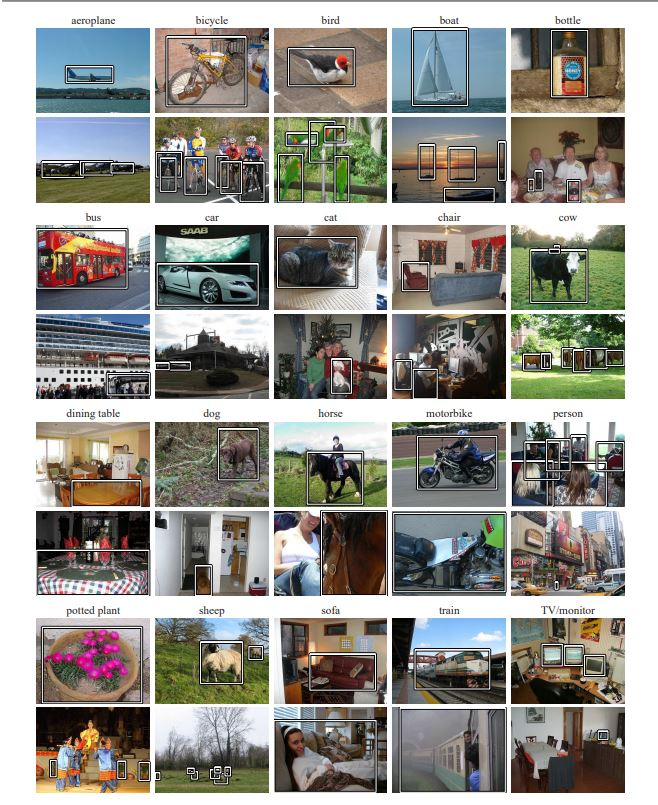
\includegraphics[width=.9\textwidth]{imagem/0x_pascal2007.jpg}
	% Caption centralizada
	\captionsetup{justification=centering}
	\captionfont{\small{\textbf{\\Fonte: \citeonline{everingham-2010}.}}}	
	\label{fig:pascal2007}
\end{figure}

\subsection{PASCAL VOC 2012}
\label{section:3:4:1}

Em 2012 foi lançado uma outra versão da \ac{PASCAL VOC}. Essa edição da competição tinha uma base de dados maior e mais robusta, embora ainda mantivesse as mesmas 20 classes da base de 2007. A Tabela \ref{tab:voc2012} mostra a distribuição de imagens e objetos na base \ac{PASCAL VOC} 2012. Nela será possível perceber o mesmo desbalanceamento encontrado na base de 2007. Porém, uma vantagem é que ela tem mais imagens, se comparada à base de 2007. Além disso, como as bases são completamente distintas, podem ser usadas em conjunto para o treinamento e a validação dos modelos.

\begin{table}[H]
	\centering
	\footnotesize
	% Alterar espaçamentos antes e depois do caption
	\setlength{\abovecaptionskip}{0pt}
	\setlength{\belowcaptionskip}{0pt}
	% Caption
	\caption[Pascal VOC 2012]{Classes de imagens do PASCAL VOC 2012}
	\label{tab:voc2012}
	\begin{tabular}{l|l|l|l|l|l|l}
		& \multicolumn{2}{l|}{Treino} & \multicolumn{2}{l|}{Validação} & \multicolumn{2}{l}{Treino/Validação} \\ \hline
		& imagens      & Objetos      & Imagens        & Objetos       & Imagens           & Objetos           \\ \hline
		Avião          & 327          & 432          & 343            & 433           & 670               & 865               \\
		Bicicleta      & 268          & 353          & 284            & 358           & 552               & 711               \\
		Pássaro        & 395          & 560          & 370            & 559           & 765               & 1119              \\
		Barco          & 260          & 426          & 248            & 424           & 508               & 850               \\
		Garrafa        & 365          & 629          & 341            & 630           & 706               & 1259              \\
		Ônibus         & 213          & 292          & 208            & 301           & 421               & 593               \\
		Carro          & 590          & 1013         & 571            & 1004          & 1161              & 2017              \\
		Gato           & 539          & 605          & 541            & 612           & 1080              & 1217              \\
		Cadeira        & 566          & 1178         & 553            & 1176          & 1119              & 2354              \\
		Vaca           & 151          & 290          & 152            & 298           & 303               & 588               \\
		Mesa de Jantar & 269          & 304          & 269            & 305           & 538               & 609               \\
		Cão            & 632          & 756          & 654            & 759           & 1286              & 1515              \\
		Cavalo         & 237          & 350          & 245            & 360           & 482               & 710               \\
		Motocicleta    & 265          & 357          & 261            & 356           & 526               & 713               \\
		Pessoa         & 1994         & 4194         & 2093           & 4372          & 4087              & 8566              \\
		Vaso de planta & 269          & 484          & 258            & 489           & 527               & 973               \\
		Ovelha         & 171          & 400          & 154            & 413           & 325               & 813               \\
		Sofá           & 257          & 281          & 250            & 285           & 507               & 566               \\
		Trem           & 273          & 313          & 271            & 315           & 544               & 628               \\
		Monitor/TV     & 290          & 392          & 285            & 392           & 575               & 784               \\
		Total          & 5717         & 13609        & 5823           & 13841         & 11540             & 27450            
	\end{tabular}
\\
\captionfont{\small{\textbf{\\Fonte: Adaptado de \citeonline{everingham-2011}.}}}
\end{table}

\subsection{Métricas}
\label{section:3:4:2}

A principal métrica utilizada para avaliar trabalhos de Localização e Classificação é a \ac{mAP}. Para deduzir o \ac{mAP}, é necessário definir os conceitos de Precisão e Revocação. Então seja $TP$ os verdadeiros positivos encontrados por um modelo, $FN$ os falsos negativos e $FP$ os falsos positivos (os verdadeiros negativos não entram no cálculo pois os modelos não são treinados com base no \textit{ground-truth} do \textit{background}). A Precisão $P$ pode ser definida pela Equação \ref{eq:eq9}.

\begin{equation}
	\label{eq:eq9}
	P = \dfrac{TP}{TP+FP}
\end{equation}

\noindent
Ao passo que a revocação $R$ pode ser definida pela Equação \ref{eq:eq10}.

\begin{equation}
	\label{eq:eq10}
	R = \dfrac{TP}{TP+FN}
\end{equation}

Uma vez que se tenha os valores de precisão e revocação, é traçada a curva $P \times R$. Essa curva se comporta com $R$ aumentando a medida que aumentam os falsos negativos e com $P$ oscilando e fazendo ``zigue-zague''. O valor teórico da Precisão média é determinado pela área sobre a curva $P \times R$ como está descrito na Equação \ref{eq:eq11}.

\begin{equation}
	\label{eq:eq11}
	AP = \int_{0}^{1}P(R)dR
\end{equation}

Porém, como mencionado anteriormente, a curva $P \times R$ se comporta de forma não-linear fazendo ``zigue-zague''. Esse comportamento dificulta um cálculo preciso da área sobre a curva. Para contornar essa dificuldade, \citeonline{salton-1986} propuseram que o valor da precisão média fosse interpolado de acordo com a Equação \ref{eq:eq12}

\begin{equation}
	\label{eq:eq12}
	AP = \dfrac{1}{11} \sum_{R_i \in \{0.0, 0.1, .. 1.0\}} max(P(R_i))
\end{equation}

\citeonline{everingham-2015} porém começaram a adotar uma forma diferente de calcular a integral a partir de 2010. Ao invés de fazer a interpolação como na Equação \ref{eq:eq12}, eles passaram a calcular a integral pela regra dos trapézios, definida pela Equação \ref{eq:eq13}.

\begin{equation}
	\label{eq:eq13}
	AP = \dfrac{0.1}{2}[P(R_0) + P(R_1) + 2.\sum_{R_i \in \{0.1, 0.2, .., 0.9\}}P(R_i)]
\end{equation}

Sendo assim, o \ac{mAP} pode ser definido como a média das precisões médias por classe.
% Nome do capítulo
\chapter{Proposta Técnica}
% Label para referenciar
\label{cap:4}
% Diminuir espaçamento entre título e texto
\vspace{-1.9cm}


\section{Metodologia}
\label{secao:4:1}

A seguir, serão definidos os passos necessários para a elaboração do trabalho proposto.

\subsection{Levantamento Bibliográfico}
\label{subsecao:4:1:1}

Nesta fase será feito um levantamento na literatura de tudo o que é julgado necessário para realizar o trabalho proposto. Será feito um estudo para compreensão da arquitetura \ac{DenseNet} \cite{liu-2017}. Além disso, serão feitos estudos com métodos da literatura como \ac{YOLO} \cite{redmon-2015}, \ac{SSD} \cite{wei-2015} e \ac{DSSD} \cite{cheng-2017}. Serão feitos também estudos para analisar o conteúdo da base de dados para testes. A base utilizada será a \ac{PASCAL VOC} \cite{everingham-2015}. Além disso, nessa etapa serão levantadas as formas de avaliar os resultados dos algoritmos.

\subsection{Testes e avaliações com métodos da literatura}
\label{subsecao:4:1:2}

Nesta etapa serão feitos os testes com os métodos já implementados na literatura. O objetivo é compreender o funcionamento, levantar os principais obstáculos nas respectivas implementações e selecionar as melhores tecnologias para a realização do projeto proposto. Nesta etapa também serão testados os algoritmos para avaliar os resultados obtidos, propostos por \citeonline{everingham-2015} e por \citeonline{lin-2014}.

\subsection{Desenvolvimento do protótipo inicial}
\label{subsecao:4:1:3}

A proposta é desenvolver um protótipo inicial usando a arquitetura da \ac{DenseNet} 121 apresentada por \citeonline{liu-2017} com alterações. As alterações a ser feitas são a remoção da camada final de classificação e a inserção de camadas intermediárias de convolução para realizar a localização dos objetos em diferentes escalas, como apresentado por \citeonline{wei-2015}. Além disso, serão aplicadas as mesmas modificações aplicadas inicialmente na \ac{ResNet} 101 para gerar o primeiro modelo proposto por \cite{cheng-2017}.

\subsection{Desenvolvimento da arquitetura final usando deconvolução}
\label{subsecao:4:1:4}

%Depois de alterar a arquitetura para fazer a detecção em múltiplas escalas usando convolução, será feita uma nova modificação da arquitetura, acrescentando camadas de deconvolução. Para cada camada de deconvolução é acrescentado um módulo de predição, que fará a localização e a classificação dos objetos. O acréscimo das camadas de deconvolução e dos novos módulos de predição seguem o modelo proposto por \citeonline{cheng-2017}.

\subsection{Avaliação dos resultados e comparação com o Estado da Arte}
\label{subsecao:4:1:5}

Por fim, erá feita a avaliação dos resultados dos métodos propostos e a comparação dos mesmos com os resultados do estado da arte. Essas avaliações serão feitas com base nas métricas que serão apresentadas na Sub-seção \ref{subsecao:4:1:1}. O objetivo é dizer o quão efetivo foi a utilização de uma arquitetura de \ac{CNN} mais moderna e avançada com métodos já conhecidos na resolução do problema de localzação e classificação.

 % \subsection{Monografia}
% \label{subsecao:4:1:6}

% Por fim será confeccionado uma monografia apresentando e descrevendo a implementação do método proposto, os resultados obtidos, uma avaliação dos resultados e uma comparação com o estado da arte.

% \section{Cronograma}
% \label{secao:4:2}

% O projeto será desenvolvido ao longo do ano 2019 seguindo o cronograma apresentado na Tabela \ref{tab:tabela1}. O período está dividido em bimestres, sendo o primeiro bimestre equivalente aos meses de janeiro e fevereiro de 2019, e assim sucessivamente.

% \begin{table}[H]
%	\centering
	% 	\vspace{-0.3cm} % espaço entre titulo e tabela
%	\caption[Cronograma de desenvolvimento]{Cronograma de desenvolvimento do projeto}
%	\label{tab:tabela1}
%	\begin{tabular}{|c|c|c|c|c|c|c|}
%		\hline
%		\multirow{2}{*}{Atividades}            & \multicolumn{6}{c|}{Bimestre} \\ \cline{2-7} 
%		& 1   & 2   & 3  & 4  & 5  & 6  \\ \hline
%		Levantamento Bibliográfico             & x   & x   & x  &    &    &    \\ \hline
%		Testes com métodos da literatura       &     &     & x  & x  &    &    \\ \hline
%		Desenvolvimento da arquitetura inicial &     &     & x  & x  &    &    \\ \hline
%		Desenvolvimento da arquitetura final   &     &     &    & x  & x  &    \\ \hline
%		Avaliação dos resultados               &     &     &    &    & x  & x  \\ \hline
%		Elaborar Monografia                    &     &     &    &    & x  & x  \\ \hline
%	\end{tabular}
%	\vspace{0.1cm} 
%	{\footnotesize\\ \textbf{Fonte: Elaborado pelo autor}}
%\end{table}


% Usar espaço para descrever base de testes, método de avaliação e fluxograma.




% PÓS-TEXTUAIS %%
% Bibliografia no arquivo 'Dissertacao.bib'
% Alterar o título das referências para somente 'Referências'
\renewcommand{\bibname}{Referências}

\bibliographystyle{abnt-alf}
\bibliography{bibliografia}
% Para forçar que os apêndices e anexos comecem no anverso
%\setboolean{@openright}{true}

%\apendice
%\begin{apendice}
%%------------------------------------------------------------------------------------------------------------------------------------------------------
% Reiniciar numeração das figuras que aparecem no apêndice
\setcounter{figure}{0}

\chapter{Primeiro apêndice}
\label{apend:codigoMpe}

% Para diminuir espaçamento entre o título e o texto
\vspace{-1.9cm}

Textos ou documentos elaborados pelo autor, como por exemplo código-fonte.


\lstinputlisting[language=C, label=codigo, caption={Trecho de código modificado}]{pos-texto/codigo.c}
%\end{apendice}

%\anexo
%% Nome do Anexo
\chapter{Primeiro Anexo}

% Para diminuir espa�amento entre o t�tulo e o texto
\vspace{-1.9cm}

% Texto
Textos ou documentos não elaborados pelo autor.

\end{document}